\documentclass[manuscript,anonymous]{acmart}
\usepackage[utf8]{inputenc}
\usepackage{algpseudocode} % for pseudocode
\usepackage{tikz} % for figures
\usepackage{subcaption} % for subfigures

\begin{document}
\title{Brief Announcement: Byzantine Eventual Consistency}
\author{Martin Kleppmann}
\email{mk428@cst.cam.ac.uk}
\orcid{0000-0001-7252-6958}
\affiliation{%
  \institution{University of Cambridge}
  \streetaddress{15 JJ Thomson Avenue}
  \city{Cambridge}
  \postcode{CB3 0FD}
  \country{UK}
}

\author{Heidi Howard}
\email{hh360@cst.cam.ac.uk}
\orcid{0000-0001-5256-7664}
\affiliation{%
  \institution{University of Cambridge}
  \streetaddress{15 JJ Thomson Avenue}
  \city{Cambridge}
  \postcode{CB3 0FD}
  \country{UK}
}

\begin{abstract}
    If more than $1/3$ of processes may be faulty, a Byzantine agreement algorithm cannot make any consistency guarantees.
    However, in such situations we can still guarantee a weaker consistency model, which we call Byzantine Eventual Consistency (BEC).
    We define BEC and introduce an algorithm that ensures this consistency model, even in a system with arbitrarily many faulty processes.
\end{abstract}
\maketitle

\section{Introduction}

Byzantine agreement assumes that at most $f$ of $n$ processes are Byzantine-faulty and without synchrony, Byzantine agreement is impossible if $n\leq3f$~\cite{Lamport:1982,Fischer:1985}.
If more than $f$ processes are faulty, neither agreement nor liveness can be guaranteed.
This is a problem because the $f$-faulty assumption is not always a realistic threat model.
Byzantine failures are not necessarily independent: if an adversary can compromise one of the processes (e.g. due to a software vulnerability), it is likely that they can compromise a majority of processes, since they are likely to all be running the same software. 
Similarly, non-malicious software bugs are likely to affect many of the processes at once.
Moreover, in some systems, the adversary may be able to spawn a large number of processes, and thus create a majority of Byzantine-faulty processes (this is known as a Sybil attack~\cite{Douceur:2002}).

This state of affairs raises the question: if Byzantine agreement cannot be achieved in the face of arbitrary numbers of Byzantine-faulty processes, what consistency model \emph{can} we achieve under that assumption?

In this paper we propose \emph{Byzantine Eventual Consistency} (BEC), a consistency model that can be achieved regardless of the number of Byzantine-faulty processes.
We define BEC in \S~\ref{sec:properties}, and in \S~\ref{sec:algorithm} we describe an algorithm that achieves BEC.
In BEC, each process is a replica of some shared state, and any two correct replicas converge towards the same state as they communicate, even if they also communicate with arbitrarily many Byzantine-faulty processes.
Essentially, we need to ensure that faulty replicas cannot corrupt the state of correct replicas.

\section{Defining Byzantine Eventual Consistency}\label{sec:properties}

Byzantine agreement is often used to decide an append-only log of values for state machine replication~\cite{Schneider:1990} (SMR) and thus requires that the following properties hold:

\begin{description}
\item[Validity:] Any value decided by a correct process must have been proposed by one of the processes.
\item[Agreement:] If two correct processes decide a value for a certain position in the log, those values are the same.
\item[Liveness:] For any value proposed, correct processes will eventually decide that value for some position in the log.
\end{description}

The agreement and liveness properties of Byzantine agreement assume that no more than $f$ processes are Byzantine-faulty, while liveness also assumes partial synchrony~\cite{Dwork:1988}.
We can define a similar set of properties for Byzantine Eventual Consistency (BEC).
These properties are weaker, but they can be satisfied without making any assumptions about the number of faulty processes or the synchrony model.
For generality, we assume each process locally maintains a monotonically growing set of updates $\mathcal{U}$.
\S~\ref{sec:smr} shows how to implement SMR using this set of updates.

\begin{description}
\item[Validity:] Any update in the set of updates of a correct process must have been proposed by one of the processes.
\item[Convergence:] When any two correct processes finish communicating, their sets of updates are the same.
\item[Liveness:] Assuming that any two correct processes will eventually finish communicating, a update proposed by one process will eventually be in the set of updates for all correct processes.
\end{description}

\section{Reconciliation algorithms}\label{sec:algorithm}

When two processes $p$ and $q$ communicate, and each process initially has updates $\mathcal{U}_p$ and $\mathcal{U}_q$ respectively, a reconciliation algorithm should ensure that both processes converge to the same set $\mathcal{U}_q \cup \mathcal{U}_q$.
The simplest reconciliation algorithm is for $p$ to send the entire set $\mathcal{U}_p$ to $q$, and for $q$ to send $\mathcal{U}_q$ to $p$, so that both processes can compute $\mathcal{U}_q \cup \mathcal{U}_q$.
However, if the sets have many elements in common, this algorithm transmits a large amount of data unnecessarily.

Non-Byzantine reconciliation algorithms often rely on vector clocks to determine which updates to send to each other~\cite{Schwarz:1994}.
However, vector clocks are not suitable in a Byzantine setting, because a faulty node could send contradictory updates to different processes using the same vector timestamp, causing two processes to have the same timestamps, but inconsistent sets of updates.
Therefore we introduce an algorithm that cannot be corrupted by faulty processes.

Let the set of updates $\mathcal{U}$ be a set of pairs $(v, \mathit{hs})$, where $v$ is any value, and $\mathit{hs}$ is a set of hashes produced by a cryptographic hash function $H(\cdot)$, such as SHA-256.
We assume that $H$ is collision-resistant (i.e.\ it is computationally infeasible to find distinct $x$ and $y$ such that $H(x) = H(y)$).

Say $\mathcal{U}$ contains updates $A = (v_A, \mathit{hs}_A)$ and $B = (v_B, \mathit{hs}_B)$, where $H(A) \in \mathit{hs}_B$.
Then we call $A$ a \emph{predecessor} of $B$, and $B$ a \emph{successor} of $A$.
Define a graph with a vertex for each update in $\mathcal{U}$, and a directed edge from each update to each of its predecessors.
We can assume that this graph is acyclic because the presence of a cycle would imply knowledge of a collision in the hash function.
Fig.~\ref{fig:example-dags} shows examples of such graphs.

Let $\mathrm{succ}^1(u)$ be the set of successors of update $u$, let $\mathrm{succ}^2(u)$ be the successors of the successors of $u$, and so on, and define $\mathrm{succ}^*(u)$ to be the transitive closure:
\[
\mathrm{succ}^i(u) =
\begin{cases}
\{( v, \mathit{hs}) \in \mathcal{U} \mid H(u) \in \mathit{hs}\} & \text{ for } i=1 \\
\bigcup_{u' \in \mathrm{succ}^1(u)} \mathrm{succ}^{i-1}(u') & \text{ for } i>1
\end{cases}
\hspace{60pt}
\mathrm{succ}^*(u) = \bigcup_{i \ge 1} \mathrm{succ}^i(u)
\]

When one process connects to another, both processes execute the algorithm in Fig.~\ref{fig:algorithm}.
We will illustrate the operation of this algorithm using the example in Fig.~\ref{fig:example-dags}; the messages sent in the course of the execution are shown in Fig.~\ref{fig:messages}.

\begin{figure}[p]
\captionsetup{justification=raggedright,singlelinecheck=false}
\begin{minipage}{0.57\linewidth}
    \hrule\vspace{4pt}
    \algblockdefx{On}{EndOn}[1]{\textbf{on} #1 \textbf{do}}{\textbf{end on}}
    \begin{algorithmic}[1]
    \On{connecting to another process}
        \State $\mathit{sent} := \{\}; \mathit{received} := \{\}$ \label{line:init}\Comment{connection-local variables}
        \State \textbf{send} $\langle\mathsf{heads}: \{H(u) \mid u \in \mathcal{U} \wedge \nexists (v, \mathit{hs}) \in \mathcal{U}.\; H(u) \in \mathit{hs}\}\rangle$ \label{line:send-heads}
    \EndOn\vspace{6pt}
    \On{receiving $\langle\mathsf{heads}: \mathit{hs}\rangle$} \label{line:recv-heads}
        \State $\mathit{reply} := \{v \mid \exists u \in \mathcal{U}.\; H(u) \in \mathit{hs} \,\wedge\, v \in \mathrm{succ}^*(u)\}$ \label{line:succ}
        \If{$\mathit{reply} \neq \{\}$}
            \State $\mathit{sent} := \mathit{sent} \cup \mathit{reply};\;$ \textbf{send} $\langle\mathsf{updates}: \mathit{reply}\rangle$ \label{line:heads-reply}
        \EndIf
        \State \Call{HandleMissing}{$\{h \in \mathit{hs} \mid \nexists u \in \mathcal{U}.\; H(u) = h\}$} \label{line:heads-missing}
    \EndOn\vspace{6pt}
    \On{receiving $\langle\mathsf{updates}: \mathit{new}\rangle$} \label{line:recv-updates}
        \State $\mathit{received} := \mathit{received} \,\cup\, \mathit{new}$ \label{line:updates-received}
        \State $\mathit{missing} := \{h \mid \exists (v, \mathit{hs}) \in \mathit{received}.\; h \in \mathit{hs} \;\wedge$ \label{line:updates-missing}
        \State \hspace{55pt}$\; \nexists u \in (\mathcal{U} \cup \mathit{received}).\; H(u) = h\}$ \label{line:updates-missing2}
        \State \Call{HandleMissing}{$\mathit{missing}$} \label{line:updates-handle-missing}
    \EndOn\vspace{6pt}
    \On{receiving $\langle\mathsf{needs}: \mathit{missing}\rangle$} \label{line:recv-needs}
        \State $\mathit{reply} := \{u \in \mathcal{U} \mid H(u) \in \mathit{missing} \wedge u \notin \mathit{sent}\}$ \label{line:needs-reply}
        \State $\mathit{sent} := \mathit{sent} \cup \mathit{reply};\;$ \textbf{send} $\langle\mathsf{updates}: \mathit{reply}\rangle$ \label{line:send-updates}
    \EndOn\vspace{6pt} \label{line:end-needs}
    \Function{HandleMissing}{$\mathit{missing}$}
        \If{$\mathit{missing} = \{\}$} \label{line:missing-empty}
            \State $\mathcal{U} := \mathcal{U} \cup \mathit{received};\;$ \textbf{finish protocol} \label{line:finish}
        \Else
            \State \textbf{send} $\langle\mathsf{needs}: \mathit{missing}\rangle$ \label{line:send-missing}
        \EndIf
    \EndFunction
    \end{algorithmic}
    \vspace{4pt}\hrule
    \caption{A reconciliation algorithm to sync updates between two processes.}\label{fig:algorithm}
\end{minipage}\hfill
\begin{minipage}{0.38\linewidth}
    \begin{subfigure}{\textwidth}
    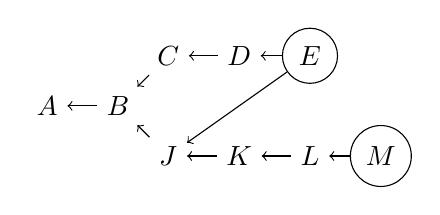
\begin{tikzpicture}[node distance=0.9cm]

% nodes
\node (a) {$A$};
\node (b) [right of=a] {$B$};
\node (c) [above right of=b] {$C$};
\node (d) [right of=c] {$D$};
\node (e) [right of=d,draw,circle] {$E$};
\node (j) [below right of=b] {$J$};
\node (k) [right of=j] {$K$};
\node (l) [right of=k] {$L$};
\node (m) [right of=l,draw,circle] {$M$};

% arrows
\draw[<-] (a) -- (b);
\draw[<-] (b) -- (c);
\draw[<-] (c) -- (d);
\draw[<-] (d) -- (e);
\draw[<-] (j) -- (e);
\draw[<-] (b) -- (j);
\draw[<-] (j) -- (k);
\draw[<-] (k) -- (l);
\draw[<-] (l) -- (m);
\end{tikzpicture}
    \caption{Graph of updates at $p$ before reconciliation}
    \end{subfigure}\\[35pt]
    \begin{subfigure}{\textwidth}
    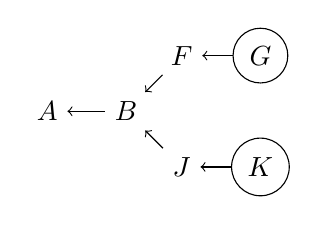
\begin{tikzpicture}

% nodes
\node (a) {$A$};
\node (b) [right of=a] {$B$};
\node (f) [above right of=b] {$F$};
\node (g) [right of=f,circle,draw] {$G$};
\node (j) [below right of=b] {$J$};
\node (k) [right of=j,circle,draw] {$K$};

% arrows
\draw[<-] (a) -- (b);
\draw[<-] (b) -- (f);
\draw[<-] (f) -- (g);
\draw[<-] (b) -- (j);
\draw[<-] (j) -- (k);
\end{tikzpicture}
    \caption{Graph of updates at $q$ before reconciliation}
    \end{subfigure}\\[35pt]
    \begin{subfigure}{\textwidth}
    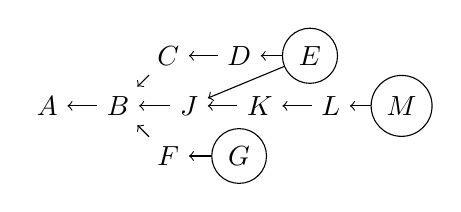
\begin{tikzpicture}[node distance=0.9cm]

% nodes
\node (a) {$A$};
\node (b) [right of=a] {$B$};
\node (c) [above right of=b] {$C$};
\node (d) [right of=c] {$D$};
\node (e) [right of=d,draw,circle] {$E$};
\node (j) [right of=b] {$J$};
\node (k) [right of=j] {$K$};
\node (l) [right of=k] {$L$};
\node (m) [right of=l,draw,circle] {$M$};
\node (f) [below right of=b] {$F$};
\node (g) [right of=f,draw,circle] {$G$};

% arrows
\draw[<-] (a) -- (b);
\draw[<-] (b) -- (c);
\draw[<-] (c) -- (d);
\draw[<-] (d) -- (e);
\draw[<-] (b) -- (j);
\draw[<-] (j) -- (e);
\draw[<-] (j) -- (k);
\draw[<-] (k) -- (l);
\draw[<-] (l) -- (m);
\draw[<-] (b) -- (f);
\draw[<-] (f) -- (g);
\end{tikzpicture}
    \caption{Graph of updates at $p$ and $q$ after reconciliation}
    \end{subfigure}
    \caption{Example DAGs of updates. Arrows represent an update referencing the hash of its predecessor, and heads (updates with no successors) are marked with circles.}
    \label{fig:example-dags}
\end{minipage}
\end{figure}

\begin{figure}[p]
    \centering
    \vspace{0.5cm}
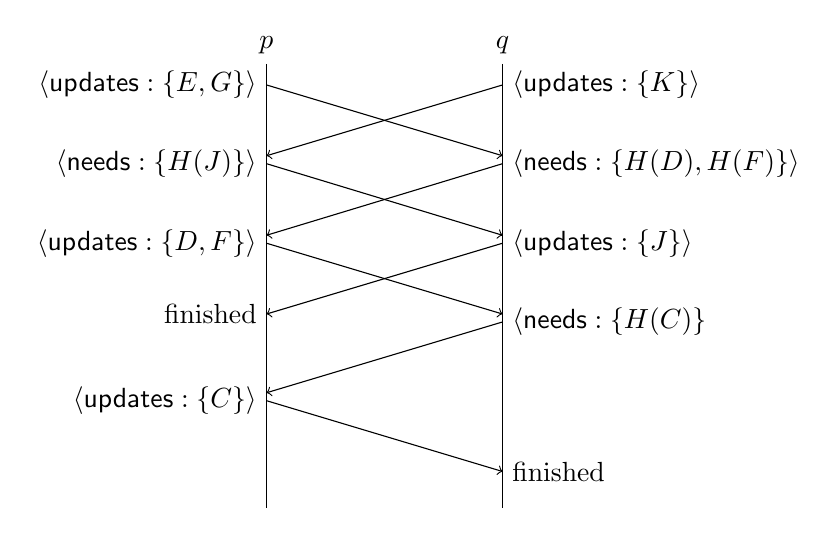
\begin{tikzpicture}
\def\width{3cm}
\def\latency{1cm}
\def\spacing{0.1cm}
\def\length{6cm}
\def\startdelay{0.5cm}

% Timelimes
\node (p1-start) at (0,0) {$p$};
\node (p2-start) at (\width,0) {$q$};
\node (p1-end) at (0,-\length) {};
\node (p2-end) at (\width,-\length) {};
\draw (p1-start) -- (p1-end);
\draw (p2-start) -- (p2-end);

% Messages
\draw[->] (0,-\startdelay) node[left] {$\langle\mathsf{updates}: \{E,G\}\rangle$} -- (\width,\spacing-\startdelay-\latency);
\draw[->] (\width,-\startdelay) node[right] {$\langle\mathsf{updates}: \{K\}\rangle$} -- (0,\spacing-\startdelay-\latency);

\draw[->] (\width, -\startdelay-\latency) node[right] {$\langle\mathsf{needs}: \{H(D), H(F)\}\rangle$} -- (0,\spacing-\startdelay-2.0\latency);
\draw[->] (0, -\startdelay-\latency) node[left] {$\langle\mathsf{needs}: \{H(J)\}\rangle$} -- (\width,\spacing-\startdelay-2.0\latency);

\draw[->] (0, -\startdelay-2.0\latency) node[left] {$\langle\mathsf{updates}: \{D, F\}\rangle$} -- (\width,\spacing-\startdelay-3.0\latency);
\draw[->] (\width, -\startdelay-2.0\latency) node[right] {$\langle\mathsf{updates}: \{J\}\rangle$} -- (0,\spacing-\startdelay-3.0\latency) node[left] {finished};

\draw[->] (\width, -\startdelay-3.0\latency) node[right] {$\langle\mathsf{needs}: \{H(C)\}$} -- (0,\spacing-\startdelay-4.0\latency);

\draw[->] (0, -\startdelay-4.0\latency) node[left] {$\langle\mathsf{updates}: \{C\}\rangle$} -- (\width,\spacing-\startdelay-5.0\latency) node[right] {finished};

\end{tikzpicture}
    \caption{Messages sent in the course of running the reconciliation algorithm in Fig.~\ref{fig:algorithm} with the example in Fig.~\ref{fig:example-dags}.}
    \label{fig:messages}
\end{figure}

Initially, when a connection is established between two processes, they send each other hashes of their \emph{heads}: that is, hashes of the updates in their local set $\mathcal{U}$ that have no successors (Fig.~\ref{fig:algorithm}, line~\ref{line:send-heads}).
In the example of Fig.~\ref{fig:example-dags}, $p$ sends $\{H(E),H(M)\}$ to $q$, while $q$ sends $\{H(G),H(K)\}$ to $p$.
Each process also initialises variables $\mathit{sent}$ and $\mathit{received}$ to contain the set of updates sent to/received from the other process within the scope of this particular connection (line~\ref{line:init}).

On receiving the head hashes from the other process (line~\ref{line:recv-heads}), the recipient first checks if its local set $\mathcal{U}$ contains successors for any of the sender's heads; if so, those successors, and any transitive successors, are sent immediately to the other process (lines~\ref{line:succ}--\ref{line:heads-reply}).
By definition of $\mathit{heads}$, these successors are not yet known to the other process.

If the recipient does not know some of the head hashes, it replies with a $\mathsf{needs}$ message requesting the updates matching those hashes (lines~\ref{line:heads-missing}, \ref{line:send-missing}).
A process responds to such a $\mathsf{needs}$ message by returning all the matching updates (lines~\ref{line:recv-needs}--\ref{line:end-needs}).
That $\mathsf{updates}$ message might again contain unresolved hashes, resulting in another $\mathsf{needs}$ message (lines~\ref{line:updates-missing}--\ref{line:updates-handle-missing}).
In successive rounds of this protocol, the processes work their way from the heads along the paths of predecessors, until they reach the updates that are common ancestors of both processes' heads.

Eventually, when there are no unresolved hashes, we merge the set of received updates into $\mathcal{U}$ and conclude the protocol run (lines~\ref{line:missing-empty}--\ref{line:finish}).
We show in the appendix that this algorithm ensures Byzantine Eventual Consistency.

\subsection{Optimisations}\label{sec:optimisations}

The algorithm in Fig.~\ref{fig:algorithm} is efficient in the sense that it does not send any updates that the other process already has.
Assuming that the number of heads is small compared to the total number of updates in $\mathcal{U}$, the initial $\mathsf{heads}$ message will be small, yielding a big performance improvement over sending the whole of $\mathcal{U}$.

In order to keep the number of heads small, whenever a correct process generates a new update $(v, \mathit{hs})$, it should set $\mathit{hs}$ to be the set of hashes of the current heads:
$\mathit{hs} = \{H(u) \mid u \in \mathcal{U} \wedge \mathrm{succ}^1(u) = \{\}\,\}$.
In this construction, the number of heads is bounded by the number of processes generating updates concurrently.
A Byzantine-faulty process may generate a large number of heads, which will affect the performance of the algorithm, but not its correctness.

A downside of the algorithm in Fig.~\ref{fig:algorithm} is that the number of round trips required can be up to the length of the longest path in the graph.
In order to optimise this, we could change lines~\ref{line:needs-reply}--\ref{line:send-updates} to send not only the immediate updates identified by the hashes in the $\mathsf{needs}$ message, but also all of the predecessors of those updates, several levels deep.
The number of round-trips is then reduced proportionally to the number of predecessor levels, but the downside is that some of the predecessors may already be known to the recipient, and are thus transmitted unnecessarily.

To determine the number of predecessor levels to send in each round, as a rule of thumb, the size of the $\mathsf{updates}$ message should be approximately equal to the bandwidth-delay product of the connection between the two processes.
Thus, on a connection with low bandwidth and fast round-trips we will prefer to send many small messages, while on a connection with high bandwidth and slow round-trips we will batch the updates into a small number of large messages.

% Prevent unbounded storage growth
% Find last common ancestor by some kind of binary search; problem: graph of updates is not linear, so definition of half-way point is fiddly.

\section{State machine replication}\label{sec:smr}

BEC can ensure convergence for any data structure that is a deterministic function of the set of updates $\mathcal{U}$.
For example, we can implement Byzantine eventually consistent state machine replication (BEC-SMR) as follows: let each value in $\mathcal{U}$ be a pair $(t, \mathit{op})$, where $t$ is a timestamp and $\mathit{op}$ is a state machine operation.
Any process may propose an operation $op$ to add to the log by generating $t$ and adding $((t, \mathit{op}), \mathit{hs})$ to $\mathcal{U}$.
The log is then simply the sequence of operations obtained by sorting the elements of $\mathcal{U}$ by timestamp, breaking ties by ordering on the hash of the respective update.

Unlike the log produced by Byzantine agreement (\S~\ref{sec:properties}), the BEC-SMR log does not guarantee that operations are added to the log in increasing timestamp order.
Thus, if a process receives operations out-of-order, it may need to roll back the state machine to an earlier state, and then replay operations in timestamp order~\cite{Jefferson:1985}.

% Can use digital signatures if you want to authenticate authors of updates

\section{Related Work}

Byzantine agreement has been subject of extensive research and has seen a recent renewal of interest due to its application in blockchains~\cite{Bano:2019}.
Many Byzantine agreement algorithms~\cite{Castro:1999,Kotla:2007,Aublin:2015} assume that $n=3f+1$ and require at least one round of communication with at least $2f+1$ processes, incurring both significant latency and limiting availability.
Zeno~\cite{Singh:2009} is able to make progress with just $f+1$ processes but instead guarantees eventual consistency.

Depot~\cite{Mahajan:2011} tolerates arbitrary numbers of faulty processes; however, its consistency model (fork-join-causal) and replication protocol are significantly more complicated than ours, making them difficult to analyse.
In BFT2F~\cite{Li:2007} and SUNDR~\cite{Mazieres:2002}, a faulty process can partition the system, preventing some processes from ever synchronising again.

Byzantine Eventual Consistency is based on \emph{Strong Eventual Consistency} (SEC)~\cite{Shapiro:2011}, a non-Byzantine consistency model in which replicas eventually converge towards the same state.
Conflict-free Replicated Data Types (CRDTs) provide SEC by ensuring that whenever any two replicas have seen the same set of updates (possibly in a different order), those replicas are in the same state~\cite{Shapiro:2011}.
We can strengthen CRDTs to provide Byzantine Eventual Consistency by making each operation an update, and using the algorithm of \S~\ref{sec:algorithm} to reconcile the sets of operations.

The hash chaining approach of our algorithm resembles a Git commit history, a blockchain~\cite{Bano:2019}, or a Merkle tree~\cite{Merkle:1987}.
Our algorithm in \S~\ref{sec:algorithm} has similarities to the protocol used by \texttt{git fetch}~\cite{GitHTTP}.
However, to our knowledge the Git protocol has not yet been the subject of much study, and particularly not in a context of Byzantine fault tolerance.


% SPORC: Group Collaboration using Untrusted Cloud Resources
% (uses fork-causal consistency)
% https://www.usenix.org/conference/osdi10/sporc-group-collaboration-using-untrusted-cloud-resources

% Secure Untrusted Data Repository (SUNDR)
% https://www.usenix.org/legacy/event/osdi04/tech/full_papers/li_j/li_j.pdf

% Roy Friedman and Roni Licher. Hardening Cassandra Against Byzantine Failures.
% https://arxiv.org/pdf/1610.02885.pdf

% Ali Shoker et al. As Secure as Possible Eventual Consistency: Work in Progress (PaPoC 2017)
% https://dl.acm.org/doi/10.1145/3064889.3064895

% Wenbing Zhao and Mamdouh Babi. Byzantine fault tolerant collaborative editing.
% https://pdfs.semanticscholar.org/587b/c024d5e877608c79f484112666489d90f041.pdf

% Git fetch negotiation algorithm, How does this compare to git fetch negotiation algorithms, default and skipping?  
% https://stackoverflow.com/questions/40484929/will-a-git-pull-develop-fetch-all-the-commits-reacheable-from-develop
% https://git-scm.com/docs/git-config#Documentation/git-config.txt-fetchnegotiationAlgorithm

% Comparison to Julien Quintard work on byzantine file systems https://www.repository.cam.ac.uk/bitstream/handle/1810/243442/thesis.pdf?sequence=1&isAllowed=y
% https://infinit.sh

% Comparison to irmin
% https://mirage.github.io/irmin/irmin/Irmin/index.html#syncing-with-a-remote
% https://github.com/mirage/irmin/blob/master/src/irmin/sync_ext.ml#L86-L123

% Comparision to byzantine quorums
% http://www.cs.cornell.edu/courses/cs5414/2017fa/papers/bquorum-dc.pdf

% Comparision to byz chain replication
% https://link.springer.com/chapter/10.1007/978-3-642-35476-2_24

\section{Conclusions}

We explore the possibilities beyond the $3f+1$ bound of Byzantine agreement.
For systems with an arbitrary number of faulty processes we propose Byzantine Eventual Consistency as a model, and a hash chaining algorithm for replication.

% We believe that a threat model with unbounded numbers of Byzantine-faulty nodes is realistic in many Internet settings, making BEC an important building block for future applications.
% We hope that future research will further develop the theory and practice of Byzantine Eventual Consistency.

\begin{acks}
Martin Kleppmann is supported by a Leverhulme Trust Early Career Fellowship, and by the Isaac Newton Trust.
\end{acks}

\bibliographystyle{ACM-Reference-Format}
\bibliography{references}

\appendix
\section{Correctness of the reconciliation algorithm}

In this appendix we show that the reconciliation algorithm of \S~\ref{sec:algorithm} satisfies the properties of Byzantine Eventual Consistency.
We consider two correct processes $p$ and $q$, with initial sets of updates $\mathcal{U}_p$ and $\mathcal{U}_q$, and final sets of updates $\mathcal{U}'_p$ and $\mathcal{U}'_q$ after they have finished communicating (i.e.\ after both processes have reached line~\ref{line:finish} of Fig.~\ref{fig:algorithm}).
We assume that $p$ and $q$ do not communicate with any other processes whilst they are communicating, nor do they add any local updates.
We use $\mathit{heads}(\mathcal{U})$ to denote the set of elements without successors in $\mathcal{U}$:
\[ \mathit{heads}(\mathcal{U}) = \{u \in \mathcal{U} \mid \nexists (v, \mathit{hs}) \in \mathcal{U}.\; H(u) \in \mathit{hs}\}. \]

\begin{lemma}\label{lemma:no-p-missing}
The set of updates of a correct process $p$ grows monotonically: $\mathcal{U}_p \subseteq \mathcal{U}'_p$.
\end{lemma}
\begin{proof}[Proof sketch.]
The process $p$ only modifies $\mathcal{U}$ by unioning it with the set $\mathit{received}$ (Fig.~\ref{fig:algorithm}, line~\ref{line:finish}), or by generating new operations, which are added to $\mathcal{U}$.
Thus, elements are only added to the set $\mathcal{U}$, and therefore $\mathcal{U}_p \subseteq \mathcal{U}'_p$.
\end{proof}

\begin{lemma}\label{lemma:no-dangling}
Let $u = (\mathit{val}, \mathit{hs})$ such that $u \in \mathcal{U}_p$.
Then for all $h \in \mathit{hs}$ we have $\exists v \in \mathcal{U}_p.\; H(v) = h$.
\end{lemma}
\begin{proof}[Proof sketch.]
There are two ways how $u$ can become a member of $\mathcal{U}_p$ for a correct process $p$:
\begin{enumerate}
    \item $u$ is generated by process $p$.
    In this case, since $p$ is assumed to be correct, $\mathit{hs} = \{H(v) \mid v \in \mathcal{U} \wedge \mathrm{succ}^1(v) = \{\}\,\}$ for some earlier state $\mathcal{U}$, as per \S~\ref{sec:optimisations}.
    As $\mathcal{U}$ grows monotonically (Lemma~\ref{lemma:no-p-missing}), $\mathcal{U} \subseteq \mathcal{U}_p$, and thus we can deduce that $\forall h \in \mathit{hs}.\; \exists v \in \mathcal{U}_p.\; H(v) = h$.
    \item $u$ is received during reconciliation with another process (which might be faulty).
    In this case, during the run of the protocol at which $p$ received $u$, we have $u \in \mathit{received}$ and $\mathit{missing} = \{\}$ at line~\ref{line:finish} of Fig.~\ref{fig:algorithm}.
    Let $\mathcal{U}$ be the set of updates at $p$ immediately before that execution of line~\ref{line:finish}.
    From $\mathit{missing} = \{\}$ and lines~\ref{line:updates-missing}--\ref{line:updates-missing2} we can deduce that $\forall h \in \mathit{hs}.\; \exists v \in (\mathcal{U} \cup \mathit{received}).\; H(v) = h$.
    Since $\mathcal{U}$ grows monotonically (Lemma~\ref{lemma:no-p-missing}) and $\mathit{received} \subseteq \mathcal{U}_p$ (line~\ref{line:finish}) we have $\forall h \in \mathit{hs}.\; \exists v \in \mathcal{U}_p.\; H(v) = h$.
\end{enumerate}
\end{proof}

\begin{lemma}\label{lemma:no-collision}
Let $u = (\mathit{val}, \mathit{hs})$ such that $u \in \mathcal{U}_p$ and $u \in \mathcal{U}_q$.
Then $\{v \in \mathcal{U}_p \mid H(v) \in \mathit{hs}\} = \{v \in \mathcal{U}_q \mid H(v) \in \mathit{hs}\}$.
\end{lemma}
\begin{proof}[Proof sketch.]
We use proof by contradiction.\\
Assume there exists $h \in \mathit{hs}$ such that $\{v \in \mathcal{U}_p \mid H(v) = h\} \neq \{v \in \mathcal{U}_q \mid H(v) = h\}$.\\
From Lemma~\ref{lemma:no-dangling} we have that $\{v \in \mathcal{U}_p \mid H(v) = h\} \neq \{\}$ and $\{v \in \mathcal{U}_q \mid H(v) = h\} \neq \{\}$.\\
Hence, there exist $v \in \mathcal{U}_p$ and $v' \in \mathcal{U}_q$ such that $v \neq v'$ and $H(v) = H(v') = h$.\\
However, this contradicts our assumption in \S~\ref{sec:algorithm} that the hash function $H(\cdot)$ is collision-resistant.
\end{proof}

\begin{lemma}\label{lemma:no-q-missing}
$\mathcal{U}_q \subseteq \mathcal{U}'_p$
\end{lemma}
\begin{proof}[Proof sketch.]
We use proof by contradiction.\\
Assume that $\exists u \in \mathcal{U}_q.\; u \notin  \mathcal{U}'_p$.\\
Since $\mathit{received}$ is a subset of $\mathcal{U}'_p$ (Fig.~\ref{fig:algorithm}, line~\ref{line:finish}) and elements are only added to $\mathit{received}$ (Fig.~\ref{fig:algorithm}, line~\ref{line:updates-received}) then $u \notin  \mathcal{U}'_p$ implies that $u \notin \mathit{received}$ on process $p$.\\
Since $u \in \mathcal{U}_q$ then either $u \in \mathit{heads}(\mathcal{U}_q)$ or $u \notin \mathit{heads}(\mathcal{U}_q)$, we now consider each case in turn.
% TODO change this to reflect that the heads message contains only hashes, no updates!
\begin{enumerate}
    \item\textsc{Case} $u \in heads(\mathcal{U}_q)$:\\
    The first message from process $q$ will be an update with $\mathit{heads}(\mathcal{U}_q)$ (Fig.~\ref{fig:algorithm}, line~\ref{line:send-heads}).\\
    Therefore $\mathit{heads}(\mathcal{U}_q) \subseteq \mathit{received}$ so $u \in \mathit{received}$ (Fig.~\ref{fig:algorithm}, line~\ref{line:updates-received}).\\
    This contradicts our previous finding that $u \notin \mathit{received}$.
    
    \item\textsc{Case} $u \notin \mathit{heads}(\mathcal{U}_q)$:\\
    Since $\mathcal{U}_q$ is a DAG and $u \notin \mathit{heads}(\mathcal{U}_q)$, there must exist an update $v$ such that $v \in \mathit{heads}(\mathcal{U}_q)$ and $v \in \mathrm{succ}^*(u)$ in $\mathcal{U}_q$.\\
    As in the previous case, $\mathit{heads}(\mathcal{U}_q) \subseteq \mathit{received}$, so $v \in \mathit{received}$.\\
    Note that none of the updates in $\mathrm{succ}^*(u)$ are in $\mathcal{U}_p$ as $u \notin \mathcal{U}'_p$ implies that  $u \notin \mathcal{U}_p$ (Lemma~\ref{lemma:no-p-missing}).\\
    If $v \in \mathrm{succ}^1(u)$ then it must the case that $u \in \mathit{received}$ by the time that $\mathit{missing} = \emptyset$, otherwise $u \in \mathit{missing}$ (Fig.~\ref{fig:algorithm}, lines~\ref{line:updates-missing}--\ref{line:updates-missing2}).\\
    By induction over the path of successors from $v$ to $u$, we observe that $u \in \mathit{received}$.\\
    At each step of the induction, the processes move to the predecessors of the previous step; due to Lemma~\ref{lemma:no-collision}, $p$ and $q$ agree about the identity of these predecessors.\\
    This contradicts our previous finding that $u \notin \mathit{received}$.
\end{enumerate}
\end{proof}

\begin{lemma}\label{lemma:no-extras}
$\mathcal{U}'_p \subseteq \mathcal{U}_p \cup \mathcal{U}_q$    
\end{lemma}
\begin{proof}[Proof sketch.]
We use proof by contradiction.\\
Assume that $\exists u \in \mathcal{U}'_p.\; u \notin \mathcal{U}_p  \land  u \notin \mathcal{U}_q$.\\
Since $\exists u \in \mathcal{U}'_p$, the process $p$ must have received an update containing $u$ from process $q$ before it finished the reconciliation algorithm (Fig.~\ref{fig:algorithm}, lines \ref{line:recv-updates}, \ref{line:updates-received}, \ref{line:finish}).\\
Process $q$ will only send an update containing $u$ if $u \in \mathcal{U}_q$ or $u \in \mathcal{U}'_q$, depending on whether process $q$ has finished the reconciliation algorithm.
Since $u \notin \mathcal{U}_q$ then process $q$ must have received an update containing $u$ from process $p$.
Since $u \notin \mathcal{U}_p$ then process $p$ will not send this message and therefore the update $u$ does not exist.
\end{proof}

\begin{theorem}\label{theorem:convergence}
When two correct processes $p$ and $q$, with initial sets of updates $\mathcal{U}_p$ and $\mathcal{U}_q$, have finished communicating (i.e.\ both have reached line~\ref{line:finish} of Fig.~\ref{fig:algorithm}), then their final sets of updates $\mathcal{U}'_p$ and $\mathcal{U}'_q$  are both equal to $\mathcal{U}_q \cup \mathcal{U}_q$.
\end{theorem}
\begin{proof}[Proof sketch.]
We can prove that $\mathcal{U}'_p = \mathcal{U}_q \cup \mathcal{U}_q$ by showing the following:
\begin{enumerate}
   \item $\mathcal{U}_p \subseteq \mathcal{U}'_p$
   \item $\mathcal{U}_q \subseteq \mathcal{U}'_p$
   \item $\mathcal{U}'_p \subseteq \mathcal{U}_p \cup \mathcal{U}_q$
\end{enumerate}

These have been shown by lemmas \ref{lemma:no-p-missing}, \ref{lemma:no-q-missing} and \ref{lemma:no-extras} respectively.  
By swapping $p$ and $q$, we can show that the same holds for $\mathcal{U}'_q$.
\end{proof}

This concludes the proof that the reconciliation algorithm of \S~\ref{sec:algorithm} satisfies the convergence property of BEC.
The proof of the validity property is obvious (the only way how an update in $\mathcal{U}$ can come into existence is by being proposed by one of the processes), and the liveness property follows from Theorem~\ref{theorem:convergence} and the assumption that any two correct processes will eventually succeed in communicating.

In this protocol, the only thing that a Byzantine-faulty process can do is to extend the set $\mathcal{U}$ with well-formed updates (i.e.\ updates containing only hashes that resolve to other updates).
If a Byzantine-faulty process generates updates containing hashes that do not resolve, the correct process will never reach the $\mathit{missing} = \{\}$ state and thus never update $\mathcal{U}$ in this protocol run.
If a faulty process responds incorrectly to a $\mathsf{needs}$ message, likewise any effects on the recipient's state are limited to well-formed updates.
This ensures the integrity of the DAG.
Arbitrary $\mathsf{needs}$ messages sent by a faulty process have no consequence, since they do not affect the state of the recipient.

% If the communication is between a correct and a Byzantine-faulty replica, the faulty replica can obviously add updates to the set or omit updates from those sent to the correct replica.
% But the faulty replica cannot corrupt the correct replica's state in a way that would prevent the correct replica from later synchronising its set of updates with another correct replica.

\end{document}
